\documentclass[pdflatex,compress]{beamer}

%\usetheme[dark,framenumber,totalframenumber]{ElektroITK}
\usetheme[darktitle,framenumber,totalframenumber]{ElektroITK}
\usepackage{graphicx}
\usepackage{multicol}

\title{Data Communications}
\subtitle{Chapter 6 - Error Detection and Correction}

\author{Mifta Nur Farid}

\begin{document}

\maketitle

\begin{frame}
	\frametitle{Types of Errors}
	\begin{itemize}
		\item An error occurs when a bit is altered between transmission and reception
		\begin{itemize}
			\item Binary 1 is transmitted and binary 0 is received
			\item Binary 0 is transmitted and binary 1 is received
		\end{itemize}
		\item \textbf{Single bit errors}
		\begin{itemize}
			\item Isolated error that alters one bit but does not affect nearby bits
			\item Can occur in the presence of white noise
		\end{itemize}
		\item \textbf{Burst errors}
		\begin{itemize}
			\item Contiguous sequence of B bits in which the first and last bits and any number of intermediate bits are received in error
			\item Can be caused by impulse noise or by fading in a mobile wireless environment
			\item Effects of burst errors are greater at higher data rates
		\end{itemize}
	\end{itemize}
\end{frame}

\begin{frame}
	\frametitle{Burst and Single-Bit Errors}
	\begin{center}
		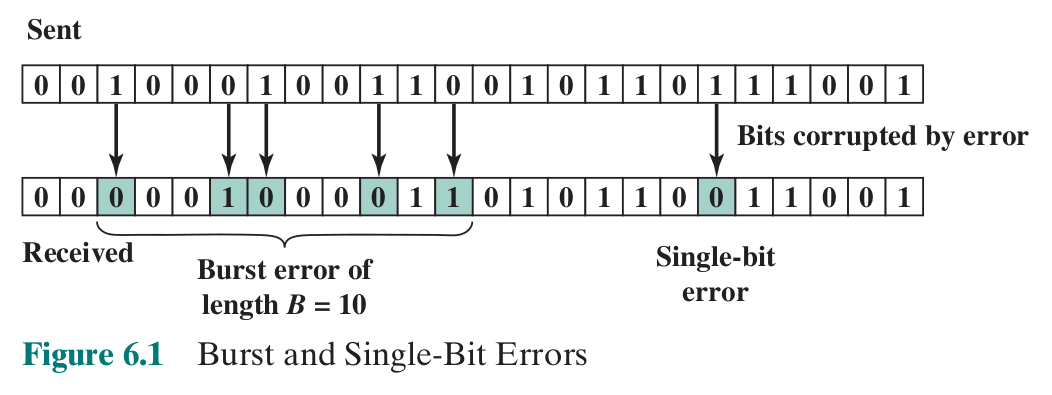
\includegraphics[width=\linewidth]{img/img01}
	\end{center}
\end{frame}

\begin{frame}
	\frametitle{Error Detection}
	\begin{itemize}
		\item Regardless of design you will have errors, resulting in the change of one or more bits in a transmitted frame
		\item Frames
		\begin{itemize}
			\item Data transmitted as one or more contiguous sequences of bits
			\item[$ P_b $ :] Probability that a bit is received in error; also known as the bit error rate (BER)
			\item[$ P_1 $ :] Probability that a frame arrives with no bit errors
			\item[$ P_2 $ :] Probability that, with an error-detecting algorithm in use, a frame arrives with one or more undetected errors
			\item[$ P_3 $ :] Probability that, with an error-detecting algorithm in use, a frame arrives with one or more detected bit errors but no undetected bit errors
		\end{itemize}
	\end{itemize}
\end{frame}

\begin{frame}{Error Detection}
	\begin{itemize}
		\item The probability that a frame arrives with no bit errors decreases when the probability of a single bit error increases
		\item The probability that a frame arrives with no bit errors decreases with increasing frame length
		\begin{itemize}
			\item The longer the frame, the more bits it has and the higher the probability that one of these is in error
		\end{itemize}
	\end{itemize}
\end{frame}

\begin{frame}
	\frametitle{Error Detection Process}
	\begin{center}
		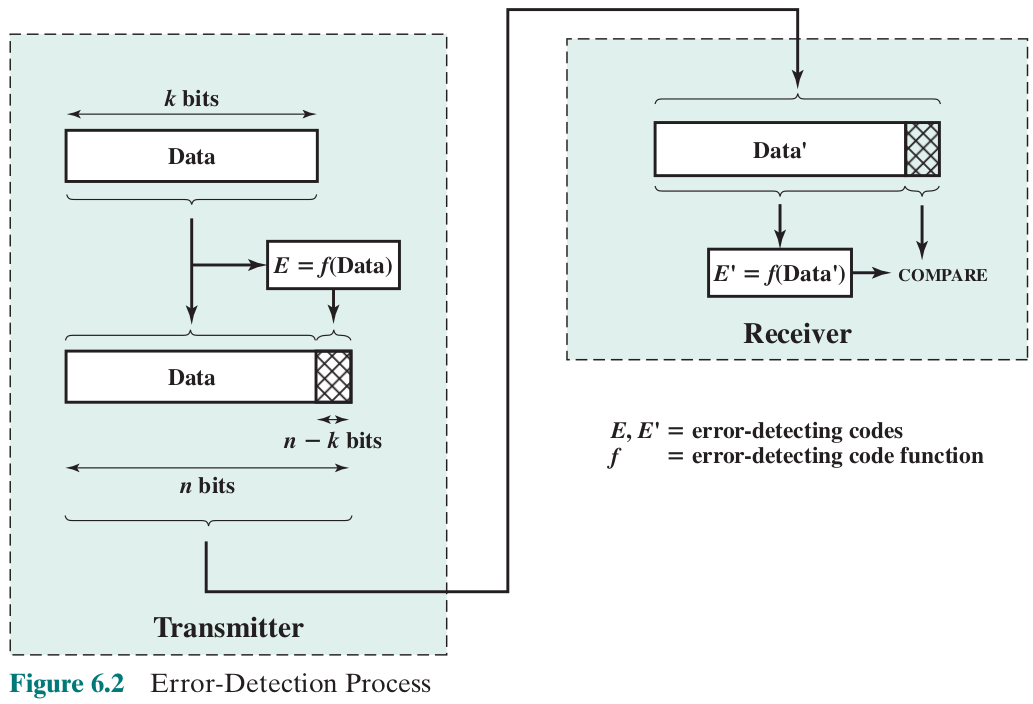
\includegraphics[width=\linewidth]{img/img02}
	\end{center}
\end{frame}

\begin{frame}
	\frametitle{Parity Check}
	\begin{itemize}
		\item The simplest error detecting scheme is to append a parity bit to the end of a block of data
		\begin{itemize}
			\item Even Parity
			\begin{itemize}
				\item Even number of 1s
				\item Used for synchronous transmission
			\end{itemize}
			\item Odd Parity
			\begin{itemize}
				\item Odd number of 1s
				\item Used for asynchronous transmission
			\end{itemize}
		\end{itemize}
		\item If any even number of bits are inverted due to error, an undetected error occurs
	\end{itemize}
\end{frame}

\begin{frame}
	\frametitle{A Two-Dimensional Even Parity Scheme}
	\begin{center}
		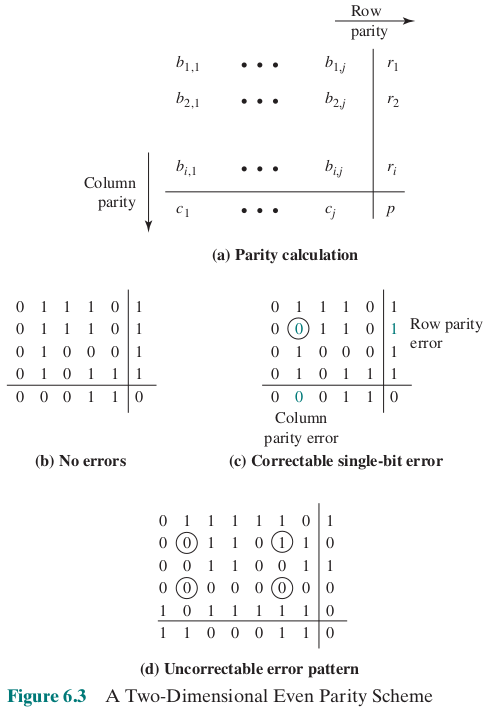
\includegraphics[height=0.8\textheight]{img/img03}
	\end{center}
\end{frame}

\begin{frame}
	\frametitle{The Internet Checksum}
	\begin{itemize}
		\item Error detecting code used in many Internet standard protocols, including IP, TCP, and UDP
		\item Ones-complement operation
		\begin{itemize}
			\item Replace 0 digits with 1 digits and 1 digits with 0 digits
		\end{itemize}
		\item Ones-complement addition
		\begin{itemize}
			\item The two numbers are treated as unsigned binary integers and added
			\item If there is a carry out of the leftmost bit, add 1 to the sum (end-around carry)
		\end{itemize}
	\end{itemize}
\end{frame}

\begin{frame}
	\frametitle{Example of Internet Checksum}
	\begin{center}
		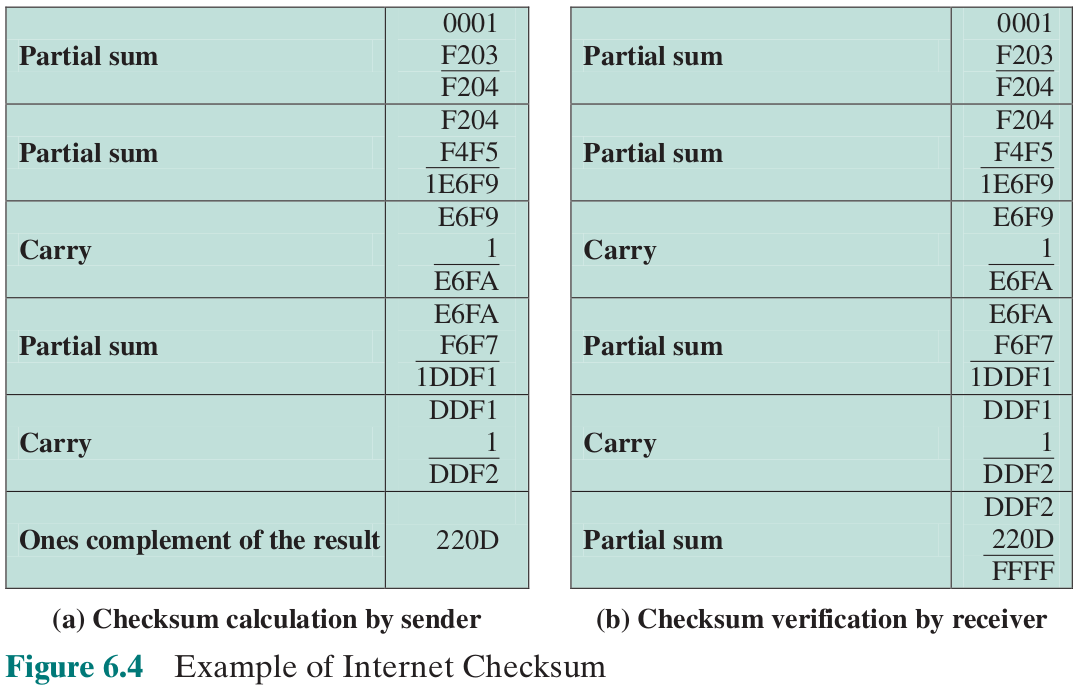
\includegraphics[width=\linewidth]{img/img04}
	\end{center}
\end{frame}

\begin{frame}
	\frametitle{Cyclic Redundancy Check}
	\begin{itemize}
		\item one of most common and powerful checks
		\item for a block of k bits transmitter generates an n bit frame check sequence (FCS)
		\item transmits k+n bits which is exactly divisible by some number
		\item receiver divides frame by that number
		\begin{itemize}
			\item if no remainder, assume no error
			\item for math, see Chapter 6
		\end{itemize}
	\end{itemize}
\end{frame}

\begin{frame}
	\frametitle{CRC Process}
	\begin{itemize}
		\item Modulo 2 arithmetic
		\begin{itemize}
			\item Uses binary addition with no carries
			\item An example is shown on page 218 in the textbook
		\end{itemize}
		\item Polynomials
		\begin{itemize}
			\item Express all values as polynomials
			in a dummy variable X, with
			binary coefficients
			\item Coefficients correspond to the bits in the binary number
			\item An example is shown on page 221 in the textbook
		\end{itemize}
	\end{itemize}
\end{frame}

\begin{frame}{CRC Process}
	\begin{itemize}
		\item Digital logic
		\begin{itemize}
			\item Dividing circuit consisting of XOR gates and a shift register
			\item Shift register is a string of 1-bit storage devices
			\item Each device has an output line, which indicates the value currently stored, and an input line
			\item At discrete time instants, known as clock times, the value in the storage device is replaced by the value indicated by its input line
			\item The entire register is clocked simultaneously, causing a 1-bit shift along the entire register
			\item An example is referenced on page 223 in the textbook
		\end{itemize}
	\end{itemize}
\end{frame}

\end{document}
